\pagebreak
\section{Affine relation is optimal for CC}

Let's assume that for every $y \in \Omega$, the relationship between intensities of images $I$ and $J$ within the window $W_y$ with center $y$, is affine:
\begin{equation}
    J(y) = \alpha_{y} I(y) + \beta_{y},
\end{equation}
for some $\alpha_{y}, \beta_{y} \in \mathbf{R}$ then the gradient of the CC metric at $x$, for any $x\in W_{y}$ is given by (eq. 4, in Avants et al.\cite{Avants2008}):
\begin{equation}
    \nabla_{x} CC(y; \psi) = \frac{2A_{y}}{B_{y}C_{y}}\left[ (I(x) - \mu_{y}) - \frac{A_{y}}{C_{y}}\left(J(\psi(x)) - \nu_{y}\right)\right]\nabla J(\psi(x)).
\end{equation}
By substituting:
\begin{equation}
    \begin{array}{lll}
        A_{y} &=& \alpha B_{y}\\
        C_{y} &=& \alpha^{2}B_{y}
    \end{array}
\end{equation}
we obtain
\begin{equation}
    \frac{A_{y}}{C_{y}}\left(J(\psi(x)) - \nu_{y}\right) =
    \frac{\alpha B_{y}}{\alpha^{2}B_{y}}\left(\alpha I(x) + \beta - \alpha \mu_{y} - \beta \right) = (I(x) - \mu_{y})
\end{equation}
which implies $\nabla_{x} CC(y; \psi) = 0$.





\section{CC gradient}
We are interested in computing the gradient of
\begin{equation}
    CC(\bar{I}, \bar{J}, x) = \frac{<\bar{I}, \bar{J}>^{2}}{<\bar{I}><\bar{J}>}
\end{equation}
where the inner product is taken over an $n^{D}$ window (eq. 4, in Avants et al.\cite{Avants2008}). Since the windows are considered discrete, a more precise notation
for this expression is:
\begin{equation}
    CC(y;\phi^{-1}_{I}, \phi^{-1}_{J}) = \frac{\left[\sum_{z\in W_{y}} \left(\tilde{I}(z) - \mu_{y}\right)\left(\tilde{J}(z) - \nu_{y}\right)\right]^{2}}
    {\left[\sum_{z \in W_{y}}\left(\tilde{I}(z) - \mu_{y}\right)^{2}\right] \left[\sum_{z \in W_{y}}\left(\tilde{J}(z) - \nu_{y}\right)^{2}\right]} = \frac{A_{y}^{2}}{B_{y}C_{y}}
\end{equation}
where $\tilde{I}(z) = I(\phi_{I}^{-1}(z))$, $\tilde{J}(z) = J(\phi_{J}^{-1}(z))$ and the full energy is given by
\begin{equation}
    CC(\phi^{-1}_{I}, \phi^{-1}_{J}) = \sum_{y\in\Omega} CC(y; \phi^{-1}_{I}, \phi^{-1}_{J})
\end{equation}
where $W_{y}$ is the window of side $n$ centered at voxel $y$, $|W_{y}|$ is the number of voxels in window $W_{y}$ and:
\begin{equation}
    \begin{array}{lll}
        \mu_{y} &=& \frac{1}{|W_{y}|}\sum_{z \in W_{y}}\tilde{I}(z)\\
        \nu_{y} &=& \frac{1}{|W_{y}|}\sum_{z \in W_{y}}\tilde{J}(z)\\
    \end{array}.
\end{equation}

We wish to compute the variation of $CC(\phi^{-1}_{I}, \phi^{-1}_{J})$ along $\phi^{-1}_{I}$ and $\phi^{-1}_{I}$, which will allow us to obtain the generalized gradients,
in a way similar to Hermosillo et al. \cite{Hermosillo2004}. We will proceed with $\phi^{-1}_{I}$, since the counterpart for $\phi^{-1}_{J}$ can be obtained analogously.
For a fixed $\phi_{J}$, define the restricted function $H(\phi_{I}) = CC(\phi_{I}, \phi_{J})$, then by differentiating w.r.t $\epsilon$ we have:
\begin{equation}
    \delta_{\psi} H(\phi^{-1}_{I}) = \left.\frac{d H(\phi^{-1}_{I} + \epsilon \psi)}{d\epsilon}\right|_{\epsilon=0} =
\end{equation}
\begin{equation}
    = \sum_{y\in\Omega}\frac{\left(2A_{y} B_{y}C_{y}\right)(\tilde{I} - \mu_{y})\left[\psi^{T}\nabla \tilde{J}\right] - 2\left(A_{y}^{2}B_{y}\right)(\tilde{J} - \nu_{y})\left[\psi^{T}\nabla \tilde{J}\right]}
                                                {B_{y}^{2} C_{y}^{2}}
\end{equation}
thus, the gradient w.r.t $\phi^{-1}_{I}$ (a function such that its inner product with $\psi$ equals the variation $\delta_{\psi} H$ for any $\psi$\cite{Hermosillo2004}) is

The set of window terms $CC(y;\phi_{I}, \phi_{J})$
that are affected by point $x$ is precisely the set of all windows $W_{y}$ such that $y \in W_{x}$. Therefore:
\begin{equation}
    \nabla_{x} CC(\phi_{I}, \phi_{J}) = \sum_{y \in W_{x}} \nabla_{x} CC(y; \phi_{I}, \phi_{J})
\end{equation}
and
\begin{equation}
    \nabla_{x} CC(y; \phi_{I}, \phi_{J}) = \frac{\left(2A_{y} B_{y}C_{y}\right)\nabla_{x}A_{y} - \left(A_{y}^{2}B_{y}\right)\nabla_{x}C_{y}}
                                                {B_{y}^{2} C_{y}^{2}}
\end{equation}
where
\begin{equation}
    \begin{array}{lll}
    \nabla_{x}A_{y} &=& (\tilde{I}(x) - \mu_{y})\nabla \tilde{J}(x)\\
    \nabla_{x}C_{y} &=& 2(\tilde{J}(x) - \nu_{y})\nabla \tilde{J}(x)
    \end{array}.
\end{equation}
Therefore, the gradient of the full energy w.r.t $x$ is
\begin{equation}
    \nabla_{x} CC(\phi_{I}, \phi_{J}) = \sum_{y \in W_{x}} \frac{2A_{y}}{B_{y}C_{y}}\left[ (\tilde{I}(x) - \mu_{y}) - \frac{A_{y}}{C_{y}}\left(\tilde{J}(x) - \nu_{y}\right)\right]\nabla \tilde{J}(x)
\end{equation}
which can be further simplified as
\begin{equation}
    \nabla_{x} CC(\phi_{I}, \phi_{J}) = \left[S_{a}(x) \tilde{I}(x) - S_{b}(x)\tilde{J}(x) - S_{c}\right]\nabla \tilde{J}(x)
\end{equation}
where
\begin{equation}
    \begin{array}{lll}
        S_{a} &=& \sum_{y \in W_{x}} \frac{2A_{y}}{B_{y}C_{y}}\\
        S_{b} &=& \sum_{y \in W_{x}} \frac{2A_{y}^{2}}{B_{y}C_{y}^{2}}\\
        S_{c} &=& \sum_{y \in W_{x}} \frac{2A_{y}}{B_{y}C_{y}} \left[ \mu_{y} - \frac{A_{y}}{C_{y}}\nu_{y}\right].
    \end{array}
\end{equation}


%
%If we assume $\phi_{I}$ and $\phi_{J}$ are initial approximations to the true transformations
%aligning $I$ and $J$, we are interested in computing two update diffeomorphisms (endomorphisms) \hbox{$\psi_{I}, \psi_{J} : \Omega_{R} \rightarrow \Omega_{R}$} such that
%
%\begin{equation}\label{eq:SyNEM_gom_update}
%    \begin{array}{ccccc}
%    	F_{J}[\tilde{J}(x)] &=& \tilde{I}(\psi_{I}(x)) &+& \eta_{J}(x)\\
%        F_{I}[\tilde{I}(x)] &=& \tilde{J}(\psi_{J}(x)) &+& \eta_{I}(x)
%    \end{array}, x\in\Omega_{R}.
%\end{equation}
%These are precisely two instances of Arce-Santana's formulation (eq. 1 of \cite{Arce-santana2014}) in the reference space, where the diffeomorphisms can be written as
%\hbox{$\psi_{I}(x) = x + \mathbf{u_{I}}(x)$}, \hbox{$\psi_{J}(x) = x + \mathbf{u_{J}}(x)$} where $\mathbf{u_{I}}$ and $\mathbf{u_{J}}$ are displacement fields.


\begin{figure}[H]
\centering
\fbox{\subfloat[Brainweb T1 (left) and T2(right) overlaid using two different channels(middle). T1 is depicted in red and T2 in green.]{\label{fig:brainweb_t1_t2_input}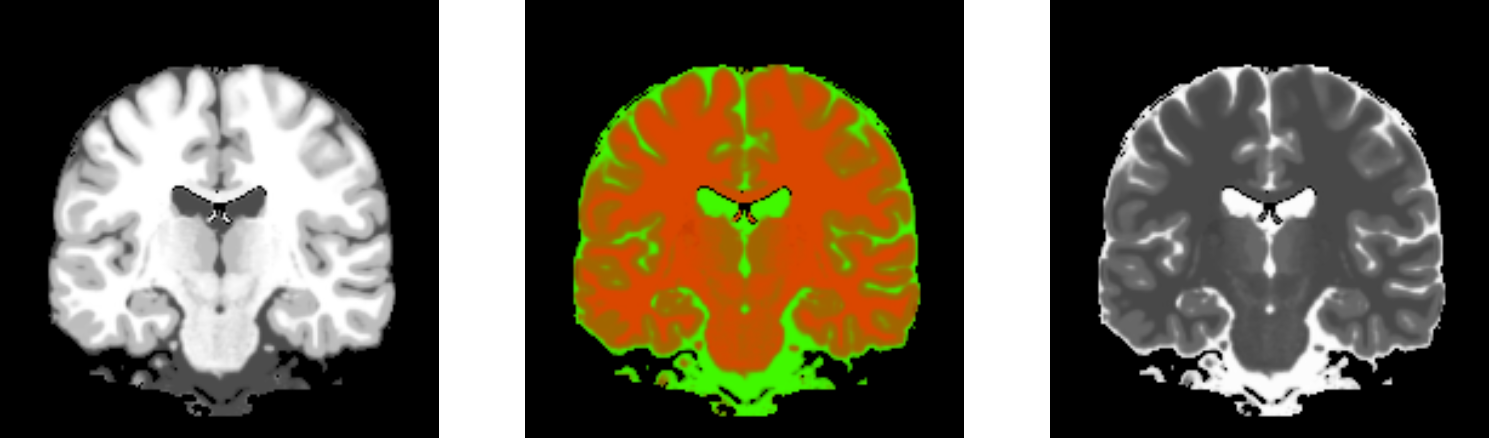
\includegraphics[width=0.8\linewidth]{./images/brainweb_t1_t2_overlay.png}}}\\
\fbox{\subfloat[T2 registered towards T1 using ANTS with the Cross-Correlation metric. Boundaries are clearly distorted.]{\label{fig:syncc_brainweb_t1_t2_overlay}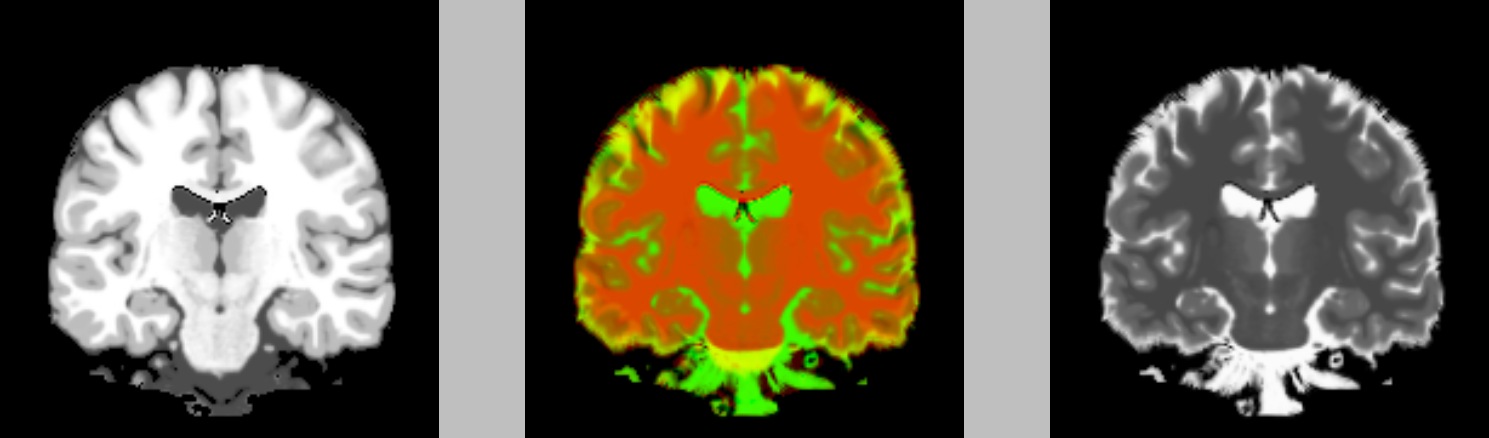
\includegraphics[width=0.8\linewidth]{./images/syncc_brainweb_t1_t2_overlay.png}}}\\
\fbox{\subfloat[T2 registered towards T1 using SyN algorithm with the Expected Cross-Correlation metric. Deformations are hard to see: ventricles are slightly dilated.]{\label{fig:syencc_brainweb_t1_t2_overlay}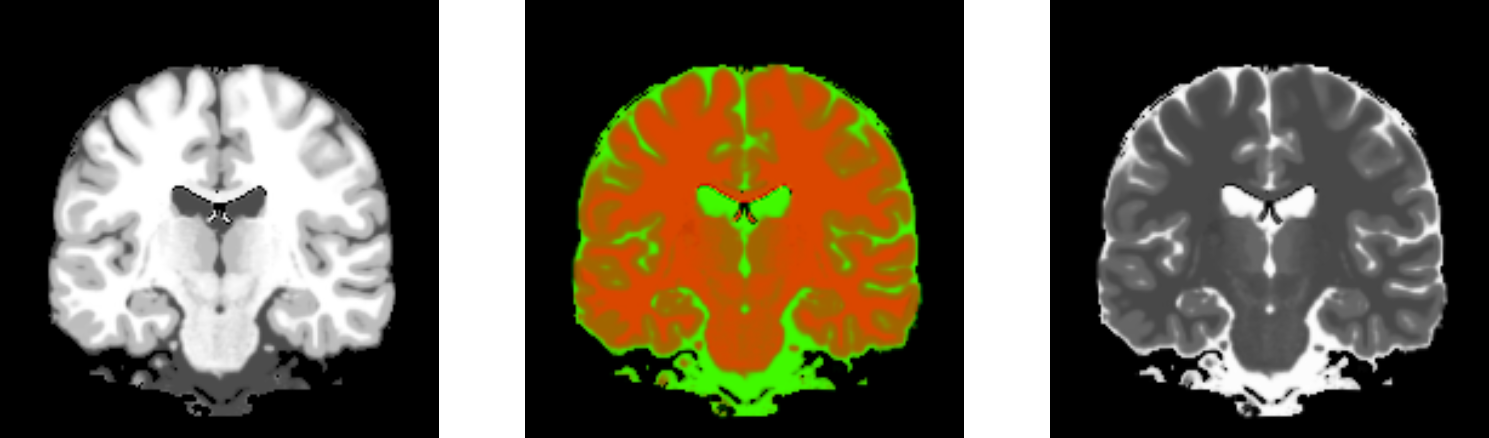
\includegraphics[width=0.8\linewidth]{./images/synecc_brainweb_t1_t2_overlay.png}}}\\
\fbox{\subfloat[Norm of displacement vectors obtained with the ECC metric. The average norm was 0.15 voxels (excluding background voxels) with a maximum of 2.6 voxels.]{\label{fig:synecc_disp_norms}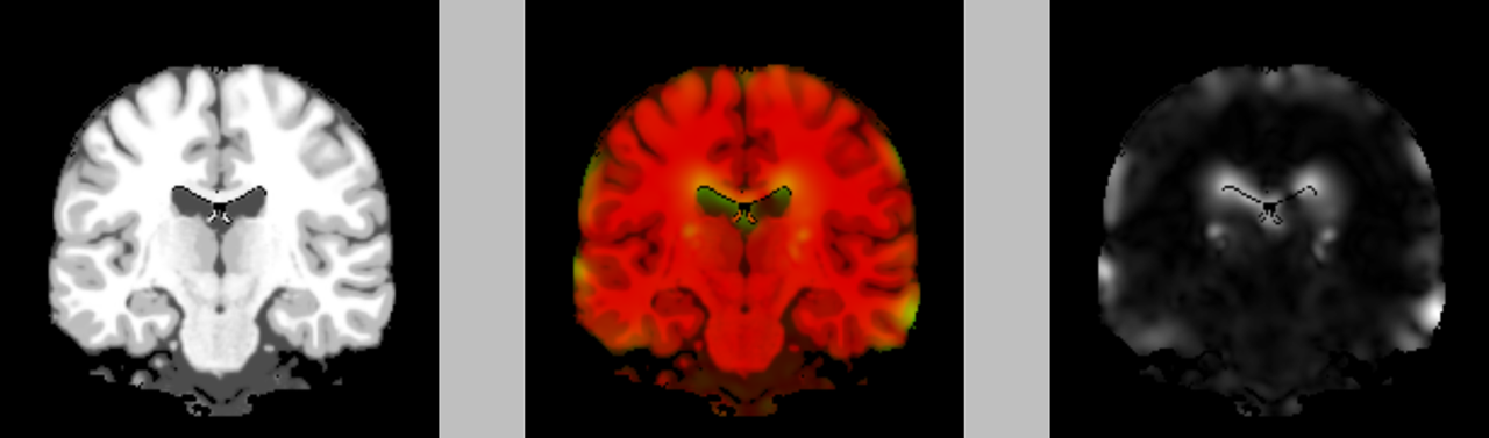
\includegraphics[width=0.8\linewidth]{./images/synecc_disp_norms.png}}}
\fbox{\subfloat[Norm of displacement vectors obtained with the MI metric. The average norm was 0.06 voxels (excluding background voxels) with a maximum of 0.4 voxels.]{\label{fig:synecc_disp_norms}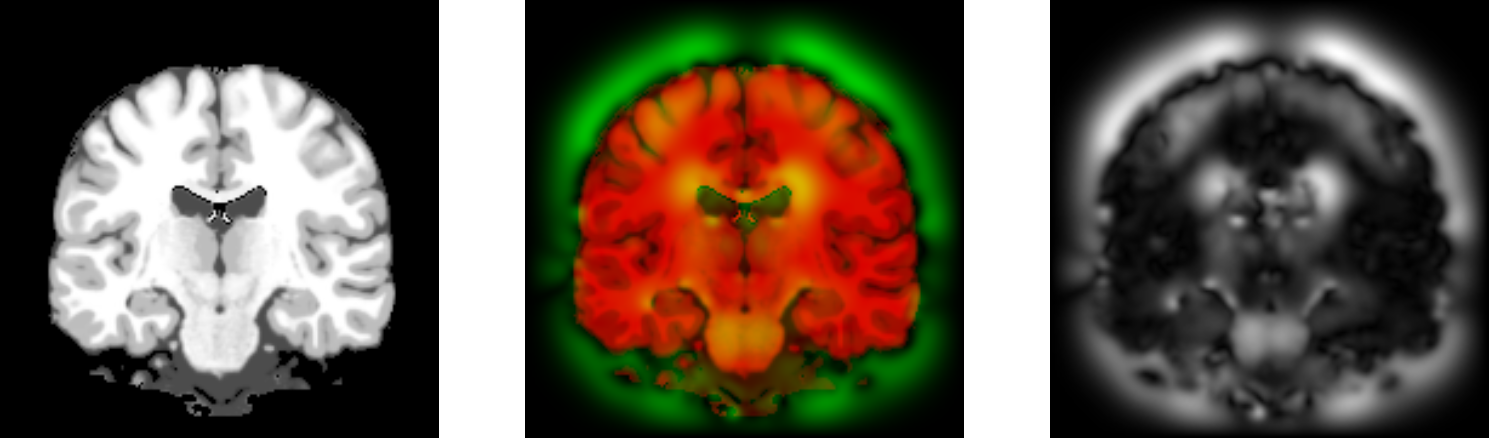
\includegraphics[width=0.8\linewidth]{./images/ants2mi_disp_norms.png}}}
\caption{Registration of two perfectly aligned images with different modalities.}
\label{fig:brainweb_t1_t2}
\end{figure}

\begin{align}
    \phi_{J}(\Omega_{J}) = \Omega_{R}\\
    \Omega_{R} = \phi_{I}(\Omega_{I})\\
    \Omega_{J} = \phi_{J}^{-1}(\phi_{I}(\Omega_{I}))\\
    \phi_{I}^{-1}(\phi_{J}(\Omega_{J})) = \Omega_{I}
\end{align}


\section{Introduction}
Introduce the topic by splitting the proble into [a] The transformation model (and cite SyN as the state of the art for registration of brain MRI), and [b] The similarity metric (and cite information-theoretic similarity metric as the most successful for multi-modal registration)
Classical Multi-modal registration algorithms: \cite{Wells1996}\cite{Maes1997}

The image intensity associated to a tissue depends on the imaging modality (T1, T2, CT) and may even depend on geometric structure and other features of the tissue (FA, MD from diffusion MRI).


Correlation-based similarity metrics are designed for situations in which the image intensities of both images are linearly correlated and work well only for mono-modal images \cite{Roche2004}.

Our algorithm presents several extensions to the algorithm proposed by Arce et al. \cite{Arce-santana2014}: (1) our resulting deformation fields are diffeomorphic, (2) we estimate both transfer functions (static to moving and moving to static), (3) we derive a demons-like step to minimize the resulting energy function, which is more efficient and easier to implement [comment: we also have the Gauss-Newton step solving the large linear system using the multi-resolution algorithm (in addition to the Gaussian pyramid), may be we can submit a version using Gauss Newton and then another one using the demons-like step].

\section{The SyN algorithm}
[briefly explain the SyN algorithm as a greedy algorithm to find the diffeomorphisms at time 0.5 and state than we are going to denote such "mid-point" diffeomorphisms as $\psi_{1}$ and $\psi_{2}$. Also explain the role of the reference domain $\Omega_R$ and state that typically it is chosen to be $\Omega{1}$, the domain of the static image.]


[Conclusion: SyNEM is very competitive, it compares favourably to FFD (one of the best performers in Klein's study \cite{Klein2009}) but still not as good as SyN with cross
correlation. This may be explained by the fact that CC uses a relatively large window centered at each voxel for computing the similarity, while the EM is voxelwise, however, note that even if the images are T1 monomodal, a naive registration using SSD is not enough because of the spatial inhomogeneities and differences in the intensity spectrum of the images (show a pair of images as an example), show the result using SSD. So, a pre-processing is necessary to match the histograms (show the results using match-histogram from ANTS), but SyNEM compares favourably against SSD with some bias correction (try the bias correction algorithm by Tustison et al.). We conclude that SyNEM is able to handle differences in the intensities of monomodal images, and partly correct bias field inhomogeneities. However it is not the best option for monomodal registration (cross correlation performs better).]




Let $I, J$ be two images defined over grids $\mathcal{L}_{I}$, $\mathcal{L}_{J}$ with grid-to-space affine transforms $\mathcal{A}_{J}, \mathcal{A}_{I}$, respectively. Let
$\phi:\Omega_{I} \rightarrow \Omega_{J}$ be a diffeomorphism where $\Omega_{I} = \mathcal{A}_{I}(\bar{\mathcal{L}_{I}})$,
and $\Omega_{J} = \mathcal{A}_{J}(\bar{\mathcal{L}_{J}})$ are the regions of $\mathbf{R}^{3}$ that are sampled by grids $\mathcal{L}_{I}$ and $\mathcal{L}_{J}$, respectively.
To ``warp'' image $J$ towards image $I$, we take each voxel $i \in \mathcal{L}_{I}$ and ``pull''the intensity value of $J$ at its corresponding point in $\mathcal{L}_{J}$
(fig. \ref{fig:pull_back}). More precisely, the warped image $\tilde{J}$ (denoted by the tilde decorator) under $\phi$, is given by
\begin{equation}\label{eq:warp_definition}
    \tilde{J}(u) = J(\mathcal{A}_{J}^{-1}\phi(\mathcal{A}_{I}u)), u \in \mathcal{L}_{I}
\end{equation}

\begin{figure}[H]
\centering
\fbox{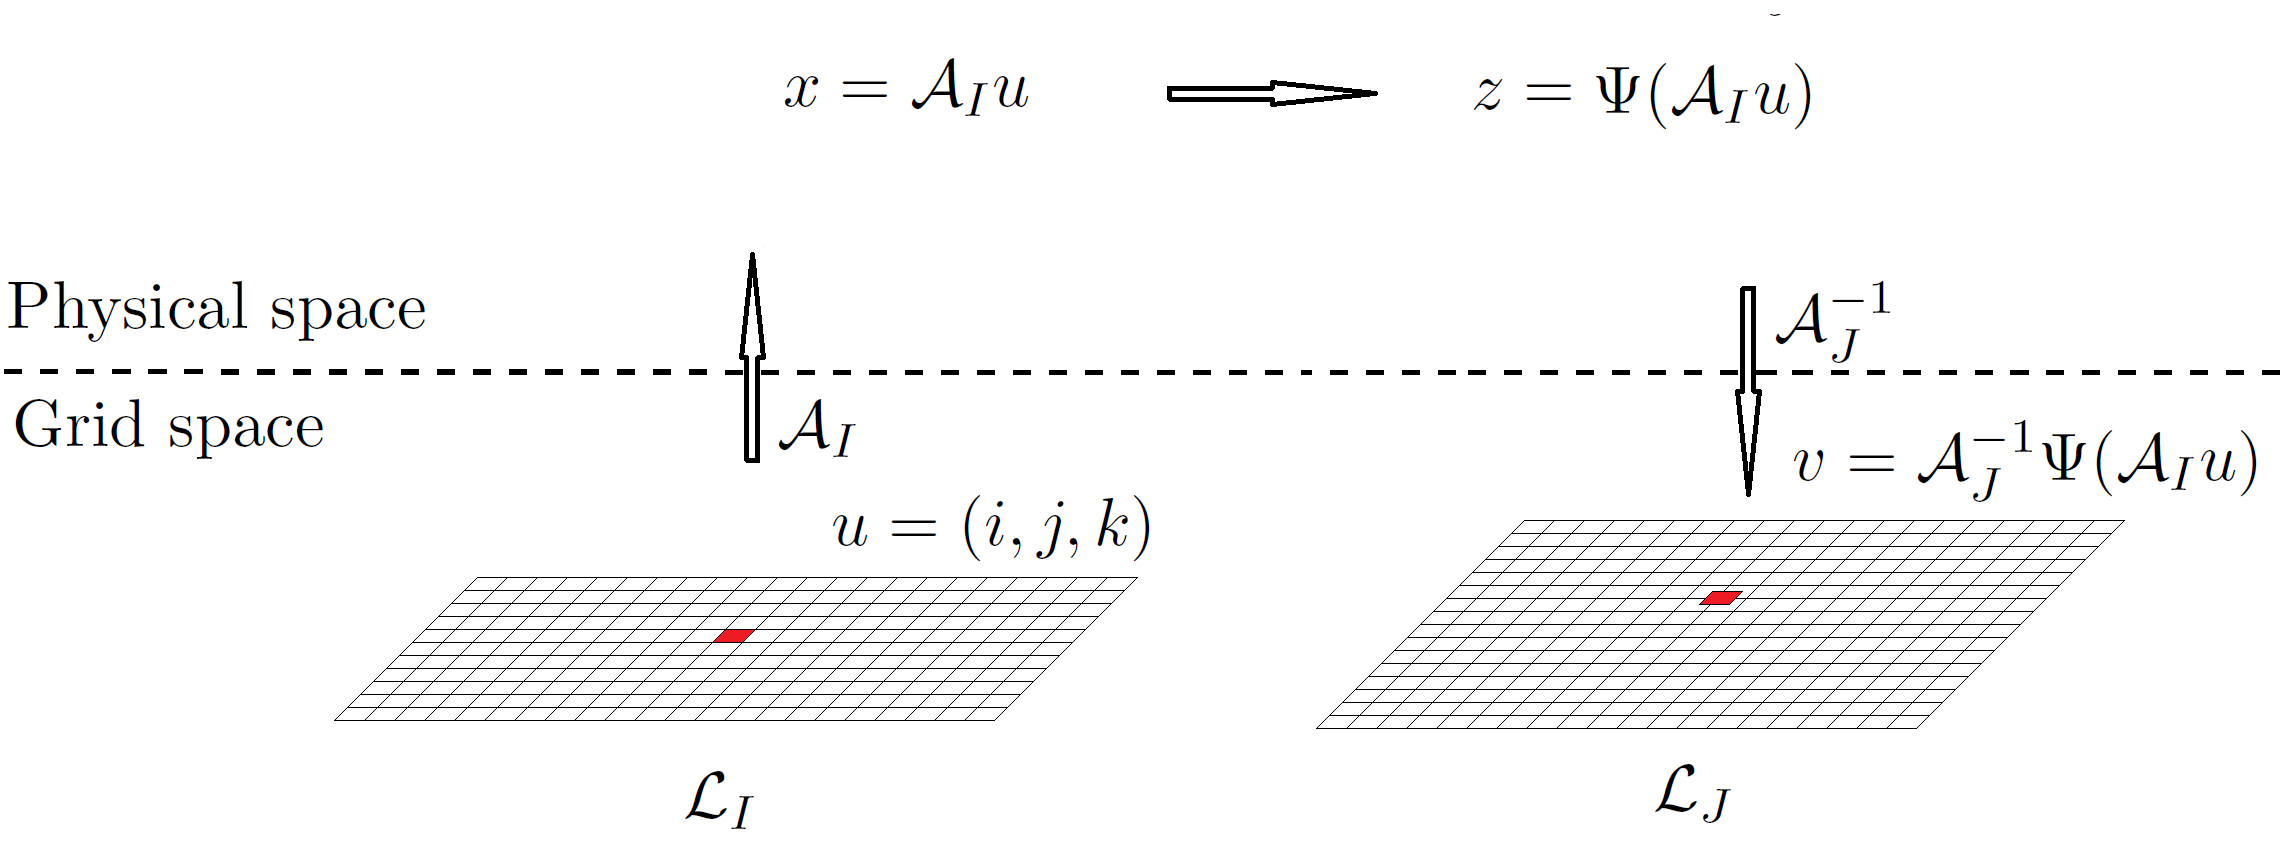
\includegraphics[width=1.0\linewidth]{./images/pull_back.png}}
\caption{Warping an image under a diffeomorphism $\phi$ is accomplished by ``pulling'' image values at $\phi$'s codomain towards its domain.}
\label{fig:pull_back}
\end{figure}


The algorithm proposed by Avants et al. \cite{Avants2011}, called {\it Greedy SyN} consists of an unconstrained search within the space of diffeomorphisms with homogeneous boundary
conditions. At each step, the Gready SyN algorithm updates the current estimate of $\psi_{1}, \psi_{2}$ by solving the Euler-Lagange equations defining necessary conditions
that the velocity fields $v_{i}$ must satisfy at each time to minimize eq. \ref{eq:syn_energy}. These equations were provided in \cite{Avants2006} for the Sum of Squared
Differences (SSD) metric as:
\begin{equation}\label{eq:euler_lagrange_ssd}
    Lv = (I - J)\nabla I.
\end{equation}

Equation \ref{eq:euler_lagrange_ssd} is important because it allows us to efficiently solve for $v$ by convolving $(I - J)\nabla I$ with the Green's kernel of the Laplacian $L$, which
is a Gaussian Kernel. Corresponding formulas to efficiently compute the update velocity fields driven by the Cross-Correlation metric were provided in \cite{Avants2009}.
Algorithm \ref{alg:Greedy_SyN} summarizes the Greedy SyN algorithm.


Even though the motivation for the greedy SyN algorithm was to find the diffeomorphisms at time 0.5 of two diffeomorphic flows in opposite directions, time does not play
any role in this algorithm. If we disregard the time component, the greedy SyN algorithm may be interpreted as a two-step registration algorithm performed in a
\textit{reference space} where the images are mapped into by composition with two diffeomorphisms as follows. Let $I$, $J$ be two images defined over $\Omega_{I}$, $\Omega_{J}$,
respectively. We consider $\Omega_{I}, \Omega_{J}$ as the transformed grids $\mathcal{L}_{I}$, $\mathcal{L}_{J}$ associated to $I, J$, under their corresponding grid-to-space
transforms $\mathcal{A}_{I}$, $\mathcal{A}_{J}$ (fig. \ref{fig:syn_overview}). Let $G$ be the set of possible intensity values these images may take
(e.g. $G=\left\lbrace 0,1,...,255\right\rbrace$). We aim to find two diffeomorphisms
$\phi_{I}:\Omega_{I}\rightarrow \Omega_{R}$, $\phi_{J}:\Omega_{J}\rightarrow \Omega_{R}$ such that the images get aligned in the reference space $\Omega_{R}$
after warping them under $\phi_{I}^{-1}$ and $\phi_{J}^{-1}$. In other words, for each point $u \in \Omega_{R}$, $I(\phi_{I}^{-1}(u))$ is mapped to $J(\phi_{J}^{-1}(u))$
(fig. \ref{fig:syn_overview}). The energy that is being minimized at each iteration is given by:

\begin{equation}\label{eq:greedy_syn_energy}
    E(v_{I}, v_{J}) = \int_{\Omega_{R}} ||\nabla v_{I}||^{2}+||\nabla v_{J}||^{2}dV + \Pi(\tilde{I}\circ v_{I}, \tilde{J}\circ v_{J})
\end{equation}











By introducing the (unknown) sets of hidden variables $Y = \left\lbrace Y_{g}=F_{I}[g] : g\in G \right\rbrace$, $Z = \left\lbrace Z_g = F_{J}[g] : g \in G\right\rbrace$ we may
apply the EM algorithm to iteratively maximize the posterior distribution
$P(\Psi | \tilde{I}, \tilde{J}) = \frac{P(\tilde{I}, \tilde{J} | \Psi)P(\Psi)}{P(\tilde{I}, \tilde{J})}$ with respect to the transformations
$\Psi = (\psi_{I}, \psi_{J})$. The estimated diffeomorphisms at iteration $t$, $\Psi^{t} = \left( \psi_{I}^{t}, \psi_{J}^{t}\right)$ can be obtained from those at iteration
$t-1$ by maximizing, with respect to $\Psi$:
\begin{equation}
	Q(\Psi, \Psi^{t-1}) = E_{Y,Z}\left[\log \left( \frac{P(\tilde{I}, \tilde{J}, Y, Z|\Psi)P(\Psi)}{P(\tilde{I}, \tilde{J}, Y, Z)}\right) | \tilde{I}, \tilde{J}, \Psi^{t-1}\right].
\end{equation}
To evaluate this expected value, we need to integrate over all possible realizations $y, z$ of the hidden variables $Y, Z$ with respect to the conditional distribution $P(y,z| \tilde{I}, \tilde{J}, \Psi^{t-1})$:
\begin{equation}\label{eq:expected_value}
Q(\Psi, \Psi^{t-1}) = \int_{y,z} (U(\Psi, y, z) - K_1)dP(y,z| \tilde{I}, \tilde{J}, \Psi^{t-1})
\end{equation}
where $K_{1} =\log P(\tilde{I}, \tilde{J}, Y, Z)$ is a normalization constant (does not depend on $\Psi$) and
\begin{align}\label{eq:SyNEM_objective}
	U(\Psi, y, z) = \log P(\tilde{I}, \tilde{J}, y, z|\Psi) + \log P(\Psi)=\\
    \nonumber\sum_{g\in G} \sum_{x : \tilde{I}(x) = g} -\frac{\left(y_g - \tilde{J}(\psi_{I}(x))\right)^{2}}{\sigma_{I}(g)^{2}} + \lambda R(\psi_{I})+\\
    \nonumber\sum_{g\in G} \sum_{x : \tilde{J}(x) = g} -\frac{\left(z_g - \tilde{I}(\psi_{J}(x))\right)^{2}}{\sigma_{J}(g)^{2}} + \lambda R(\psi_{J}).
\end{align}
The regularization functional $R(\cdot)$ encode our prior knowledge about $\Psi$ by $\log P(\Psi) = \lambda \left( R(\psi_{I}) + R(\psi_{J})\right)$ where $\lambda > 0$ is a parameter controlling the amount of regularization.\\

If we assume $Y$ and $Z$ are independent, and their elements $Y_g$ and $Z_g$, $g\in G$ are independent from each other, then the density function $P(y,z| I, J, \Psi^{t-1})$ can be written as the product of two separate densities
\begin{equation}\label{eq:density_products}
    P(y,z| I, J, \Psi^{t-1}) = h_{Y}(y)h_{Z}(z) = \prod_{g\in G}h_{Y_g}(y_g) \prod_{g\in G}h_{Z_g}(z_g),
\end{equation}
and the expected value (eq. \ref{eq:expected_value}) can be written as
\begin{align}
    -K_{1}-\int\sum_{g\in G} \sum_{x : I(x) = g} \frac{\left(y_g - \tilde{J}(\psi_{I}(x))\right)^{2}}{\sigma_{I}(g)^{2}}d h_{Y}(y)-\\
    \nonumber\int\sum_{g\in G} \sum_{x : J(x) = g} \frac{\left(z_g - \tilde{I}(\psi_{J}(x))\right)^{2}}{\sigma_{J}(g)^{2}}d h_{Z}(z)
\end{align}
which can be further simplified (by using eq. \ref{eq:density_products} to split the densities $h_{Y}(y)$ and $h_{Z}(z)$ as products of individual densities for each intensity $g \in G$) as
\begin{align}
    -K_{1}-\sum_{g\in G} \sum_{x : I(x) = g} \int\frac{\left(r - \tilde{J}(\psi_{I}(x))\right)^{2}}{\sigma_{I}(g)^{2}}d h_{Y_g}(r)-\\
    \nonumber\sum_{g\in G} \sum_{x : J(x) = g} \int\frac{\left(s - \tilde{I}(\psi_{J}(x))\right)^{2}}{\sigma_{J}(g)^{2}}d h_{Z_g}(s)
\end{align}
now let $\bar{r}(g)$ and $\bar{s}(g)$ be the expected value of $Y_g$ and $Z_g$ given $I, J, \Psi^{t-1}$ respectively, then
\begin{align}
    &\int\left(r - \tilde{J}(\psi_{I}(x))\right)^{2}d h_{Y_g}(r) = &\\
    &\nonumber \int\left(r - \bar{r}(g) + \bar{r}(g) - \tilde{J}(\psi_{I}(x))\right)^{2}d h_{Y_g}(r) = &\\
    &\nonumber \sigma^{2}_{I}(g) + \int\left(\bar{r}(g) - \tilde{J}(\psi_{I}(x))\right)^{2}d h_{Y_g}(r) = &\\
    &\nonumber \sigma^{2}_{I}(g) + \left(\bar{r}(g) - \tilde{J}(\psi_{I}(x))\right)^{2}&
\end{align}
because $h_{Y_g}$ is a density function and we are integrating over its entire domain. Analogously:
\begin{align}
    \int\left(s - \tilde{I}(\psi_{J}(x))\right)^{2}d h_{Z_g}(s) = \sigma^{2}_{J}(g) + \left(\bar{s}(g) - \tilde{I}(\psi_{J}(x))\right)^{2}
\end{align}

Now let's denote by $\hat{\mu}_{I}(x) = \bar{r}(\tilde{I}(x))$, $\hat{\sigma}_{I}(x) = \sigma_{I}(\tilde{I}(x))$ and analogously
$\hat{\mu}_{J}(x) = \bar{s}(\tilde{J}(x))$, $\hat{\sigma}_{J}(x) = \sigma_{J}(\tilde{J}(x))$, in other words, we assign to each voxel $x$ from
$\tilde{I}$ the expected value $\bar{r}(g)$ corresponding to the intensity $g$ of $\tilde{I}$ at $x$ and denote it by $\hat{\mu}_{I}(x)$, assign
its corresponding variance and denote it by $\hat{\sigma_{I}}(x)$ and proceed analogously for $\hat{\mu}_{J}(x)$ and $\hat{\sigma}_{J}(x)$ using $J$.
Then, the expected value that needs to be maximized in the M-step of the EM algorithm (eq. \ref{eq:expected_value}) can be written as:
\begin{align}\label{eq:SyNEM_objective}
    -Q(\Psi, \Psi^{t-1}) = \sum_{x \in \Omega_{I}} \frac{(\hat{\mu}_{I}(x) - \tilde{J}(\psi_{I}(x)))^{2}}{\hat{\sigma}_{I}(x)} + \lambda R(\psi_{I}) + \\
    \nonumber\sum_{x \in \Omega_{J}} \frac{(\hat{\mu}_{J}(x) - \tilde{I}(\psi_{J}(x)))^{2}}{\hat{\sigma}_{J}(x)} + \lambda R(\psi_{J})
\end{align}

The main difficulty of directly minimizing eq. (\ref{eq:SyNEM_objective}) is that both similarity terms depend on both diffeomorphisms
$\psi_{I}$ and $\psi_{J}$ since $\tilde{J}(\psi_{I})$ depends on $\psi_{J}^{-1}$ and $\tilde{I}(\psi_{J})$ depends on $\psi_{I}^{-1}$, which implies that the
objective function must be optimized with respect to both diffeomorphisms simultaneously, which is very challenging because an explicit formula for the representation
of $\psi_{I}^{-1}$ and $\psi_{J}^{-1}$ in terms of the parameters of $\psi_{I}$ and $\psi_{J}$ may not be available or may be prohibitively costly to compute
\footnote{Diffeomorphisms are typically parameterized by displacement fields (a displacement vector for each voxel) and the problem of inverting a displacement field
has been subject of substantial research. All available methods for approximating displacement field inverses are iterative, see for example:
\cite{Chen2008}\cite{Avants2009}\cite{Christensen2001}\cite{Crum2007}\cite{Yan2010}}. To overcome this difficulty, the greedy SyN algorithm proposed by Avants et al.
\cite{Avants2011} uses the inverses at iteration $t-1$ to compute $\tilde{I}$ and $\tilde{J}$, then updates the direct transformations at iteration $t$ and updates the
inverses at iteration $t$ by inverting $\psi_{I}^{t}$ and $\psi_{J}^{t}$ using a variation of the fixed point algorithm proposed by Chen et al.\cite{Chen2008} (see
algorithm \ref{alg:SyNEM}). This scheme has the extra advantage that both similarity terms are now decoupled.\\



\section{Gauss-Newton Step}

\section{Demons Step}
After modeling the transfer function from voxel intensities in the static image to voxel intensities in the moving image, we obtain the following energy function that needs to be minimized to obtain the optimal displacement filed (eq. 22 of \cite{Arce-santana2014}):


Recent tractography methods use anatomical information to improve tracking [need references to anatomically enhanced tractography methdods], these methods require a way of mapping
anatomical features computed from high-resolution T1 images to diffusion data, and this mapping is obtained by multi-modal registration. Even though the multi-modality images
correspond to the same subject, dMRI data contain geometric distortions produced by magnetic field susceptibility [references needed] and Eddy currents [references needed], thus,
in general, affine registration is insufficient to correctly register the images. Mapping dMRI to T1 is important too: observe the location of the tracts on the anatomy.
